\section{Background subtraction}

We have implemented an algorithm to segment a video into different shots. It bases its functionality on the absolute difference between histograms of frames. We are dealing with color images and we do not want to use the color information to help in the detection of shot transitions. Therefore for each image we concatenate the histograms of the three channels into a single vector. For each image we sum the absolute differences of its histogram vector and the former one. Our algorithm detects a shot transition for each of the peaks in the differences progression. In order to avoid spurs we impose a minimum height for a peak in order to be selected. We have chosen empirically a height of 200000. We also impose a minimum distance of 10 frames between consecutive peaks. Figure \ref{fig:history-differences} shows the evolution of the histogram difference between each frame and the former one. We have also marked the peaks that have been selected by our algorithm as shot transitions.

\begin{figure}[htb]
\centering
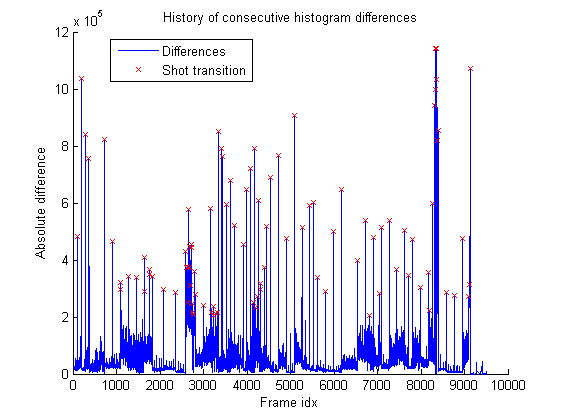
\includegraphics[width=0.6\textwidth]{./img/ex1/history-differences.png}
\caption{History of absolute differences between consecutive histograms}
\label{fig:history-differences}
\end{figure}

After the shot transitions have been identified we try to infer the background of those shots in which the camera is static. To do so we calculate the component-wise median of the color for each pixel in the shot. Then this background is used to extract the moving objects of the scene, this is, the foreground. We can see in figure \ref{fig:background-subtraction} some examples for different shots.

\begin{figure}[htb]
	\centering
	\begin{subfigure}[t]{0.65\textwidth}
		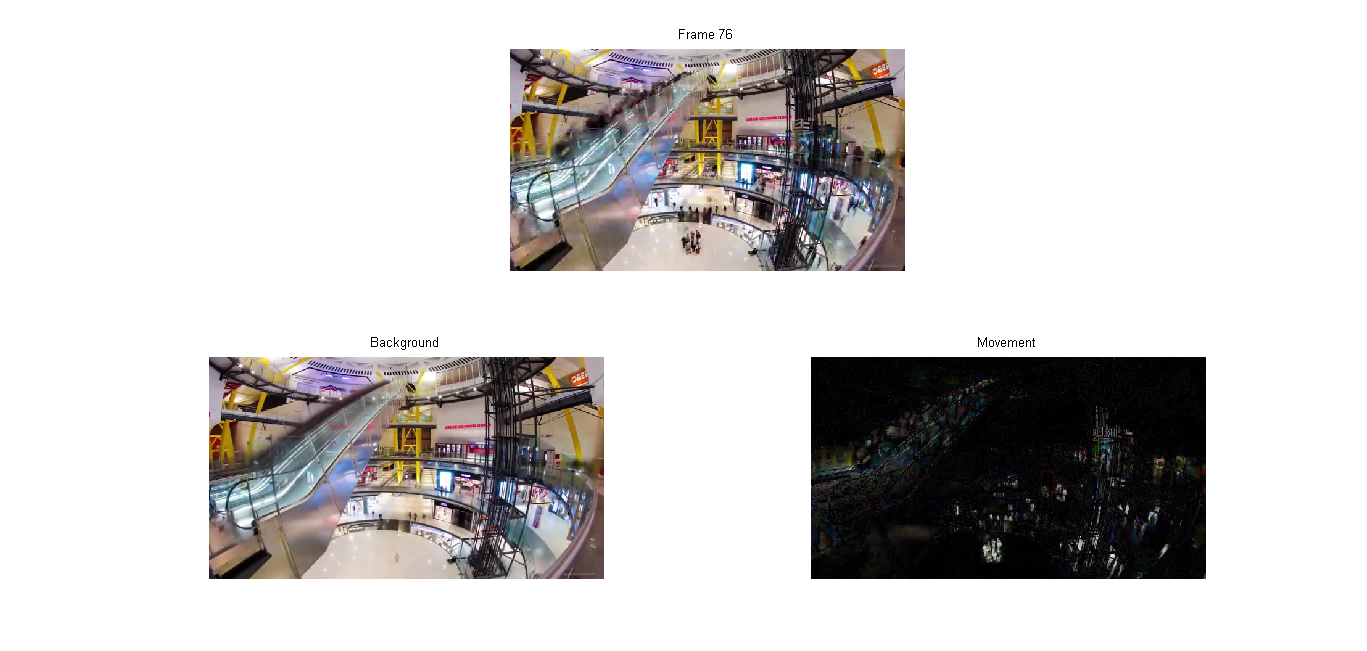
\includegraphics[width=\textwidth]{./img/ex1/shot1.png}
		\caption{Shot from 0:29 to 0:35}
		\label{fig:shot1}
	\end{subfigure}
	
	\begin{subfigure}[t]{0.65\textwidth}
		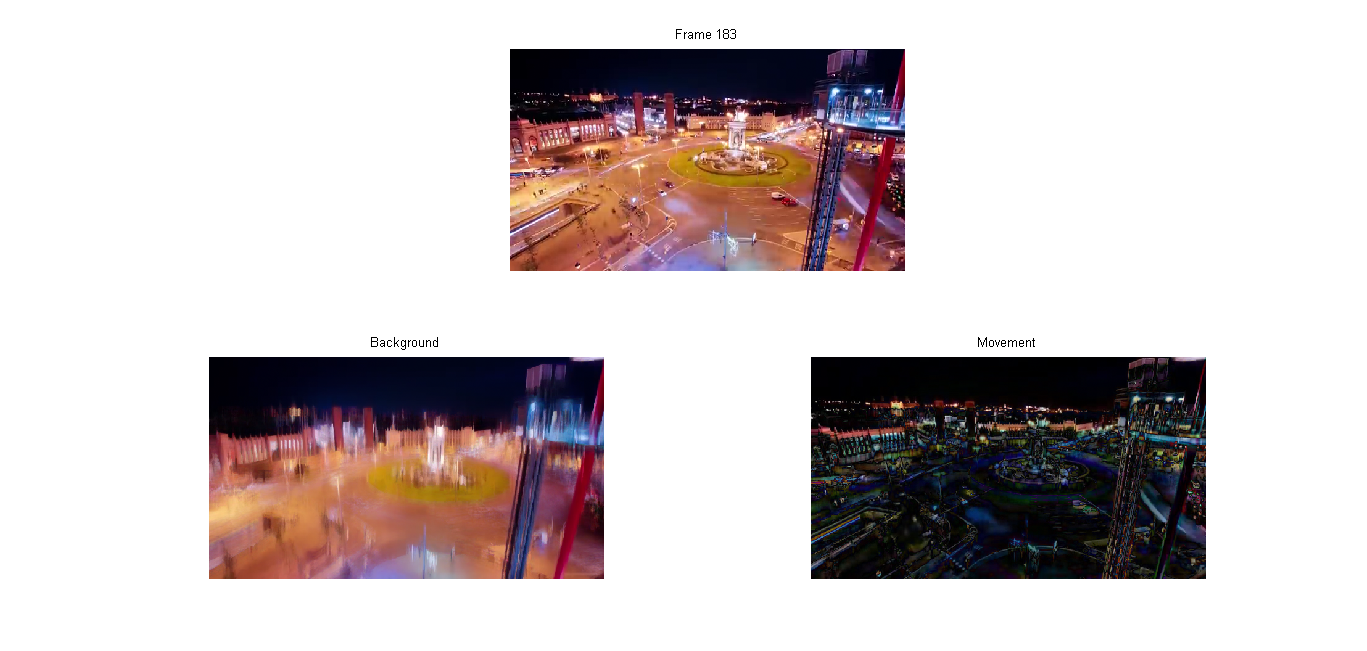
\includegraphics[width=\textwidth]{./img/ex1/shot2.png}
		\caption{Shot from 0:35 to 0:39}
		\label{fig:shot2}
	\end{subfigure}
	
	\begin{subfigure}[t]{0.65\textwidth}
		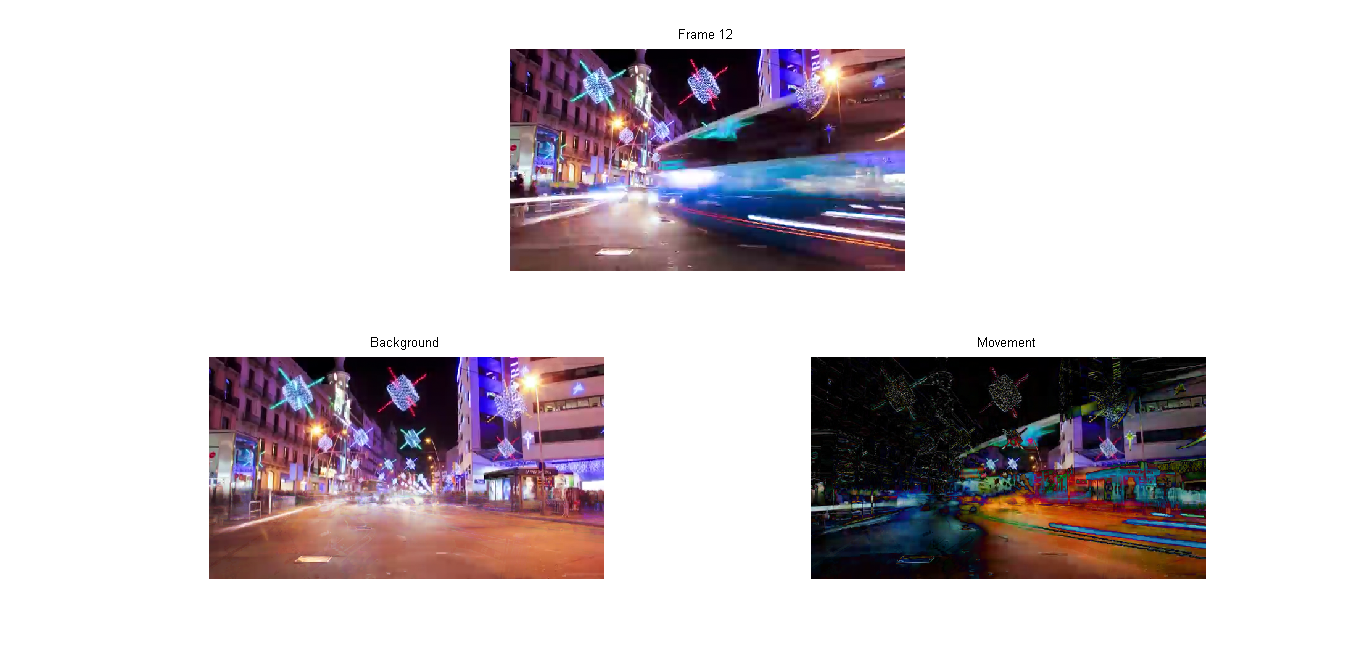
\includegraphics[width=\textwidth]{./img/ex1/shot3.png}
		\caption{Shot from 0:39 to 0:43}
		\label{fig:shot3}
	\end{subfigure}
	
	\begin{subfigure}[t]{0.65\textwidth}
		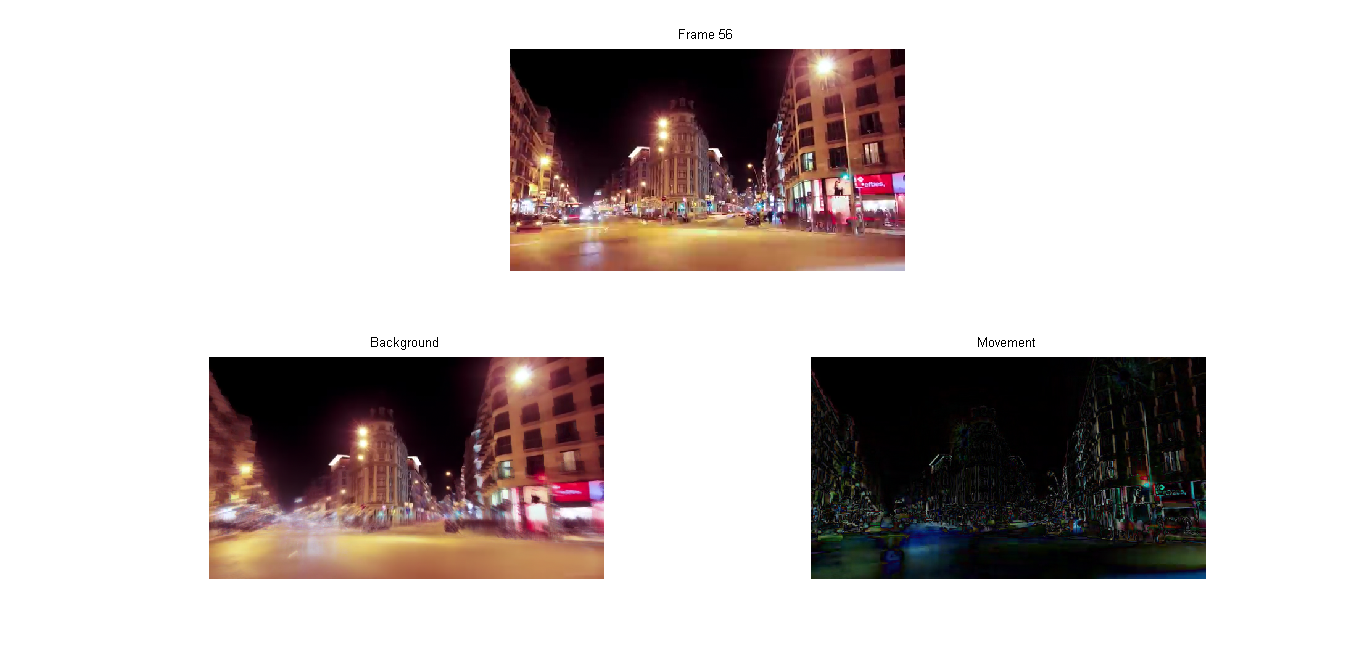
\includegraphics[width=\textwidth]{./img/ex1/shot4.png}
		\caption{Shot from 0:50 to 0:58}
		\label{fig:shot4}
	\end{subfigure}
	
\caption{Examples of background extraction for different shots}
\label{fig:background-subtraction}
\end{figure}

Notice that in the shot \ref{fig:shot1} the camera is completely static and the background extraction yields pretty good results. However, in the shots \ref{fig:shot2} and \ref{fig:shot4} there is some blurring in the extracted background due to the fact that the camera is panning and zooming out, respectively. The case of \ref{fig:shot3} is special. While the actual shot is longer and there is a slow zoom out there has been a bit of oversegmentation due to the sudden appearance of the bus. In balance the inferred background is quite sharp thanks to the short duration of the extracted shot.

We believe that it is preferable to have some oversegmentation rather than different shots recognized as a single one. Therefore we conclude that the implemented algorithm has good applicability to video segmentation whenever sudden transitions are used. On the other hand the background extraction strategy can have its applications for surveillance or in the film industry (the famous ``green'' backgrounds).

The code used for this section is available in the \texttt{video\_segmentation.m} and the \texttt{play\_shot.m} functions. In order to learn more, we refer the reader to the annex and to the source itself.

\FloatBarrier
